\documentclass[11pt]{article}
\usepackage{graphicx,fancyhdr,amsmath,amssymb,amsthm,subfig,url,hyperref}
\usepackage[margin=1in]{geometry}
\usepackage{placeins}
%----------------------- Macros and Definitions --------------------------

%%% FILL THIS OUT
\newcommand{\studentname}{Pramesh Kumar}
\newcommand{\suid}{kumar372}
\newcommand{\exerciseset}{Instructions for installing Python and Gurobi}
%%% END



\renewcommand{\theenumi}{\bf \Alph{enumi}}

%\theoremstyle{plain}
%\newtheorem{theorem}{Theorem}
%\newtheorem{lemma}[theorem]{Lemma}

\fancypagestyle{plain}{}
\pagestyle{fancy}
\fancyhf{}
\fancyhead[RO,LE]{\sffamily\bfseries\large University of Minnesota}
\fancyhead[LO,RE]{\sffamily\bfseries\large CEGE 4011/5214: Transportation Systems Analysis}
\fancyfoot[LO,RE]{\sffamily\bfseries\large \studentname: \suid @umn.edu}
\fancyfoot[RO,LE]{\sffamily\bfseries\thepage}
\renewcommand{\headrulewidth}{1pt}
\renewcommand{\footrulewidth}{1pt}

\graphicspath{{figures/}}

%-------------------------------- Title ----------------------------------

\title{\exerciseset}
\author{\studentname \qquad x500: \suid}

%--------------------------------- Text ----------------------------------

\begin{document}
	\maketitle
	
	\section*{1. Installing Python}
	There are various ways of installing python. The straightforward way is to go to the website \href{https://www.python.org/downloads/}{https://www.python.org/downloads/} and download the installer and install python. Another way is to install Anaconda which installs Python with an Integrated Development Environment (IDE) named \textbf{Spyder}, a command shell named \textbf{IPython}, and \textbf{Jupyter Notebook}, which I'll use for teaching.
	
	\subsection*{What is Anaconda?}
	According to Wiki, Anaconda is a free and open-source distribution of the \textbf{Python} and \textbf{R} programming languages for scientific computing (data science, machine learning applications, large-scale data processing, predictive analytics, etc.), that aims to simplify package management and deployment. 
	
	\subsection*{Instructions to install Anaconda}
	\begin{enumerate}
		\item Go to the website \href{https://www.anaconda.com/products/individual}{https://www.anaconda.com/products/individual}.
		\item Click on the \textbf{Download} button. Then, select the appropriate OS and processor (See Figure \ref{fig:install}) and save the installer file. 
		
		\begin{figure}[h!]
			\centering
			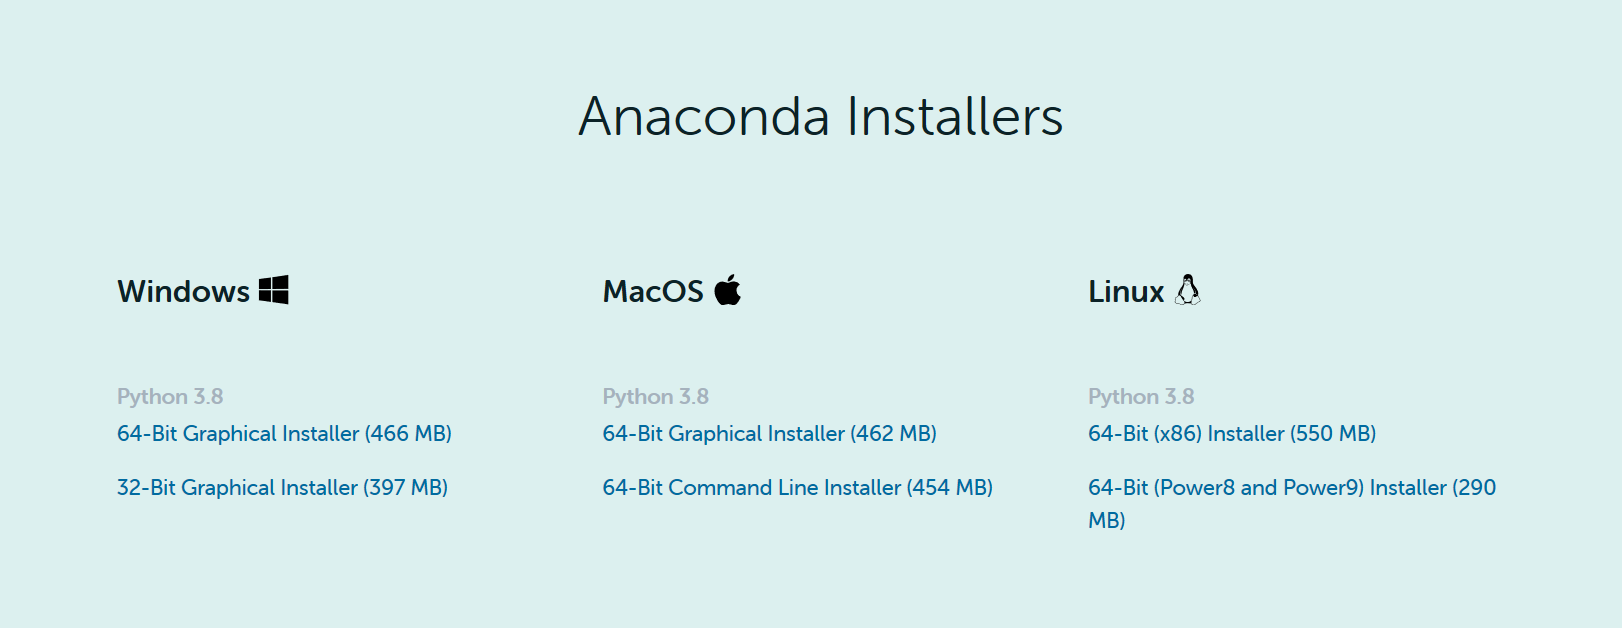
\includegraphics[width=1\linewidth]{Fig/down.png}
			\caption{Available installers}
			\label{fig:install}
		\end{figure}
		\item Go to the download folder location and double click on the installer.
		\item Click \textbf{ Next, I agree, Next}, then \textbf{Install}, and finally, \textbf{Finish}. 

		\begin{figure}[h!]
			\centering
			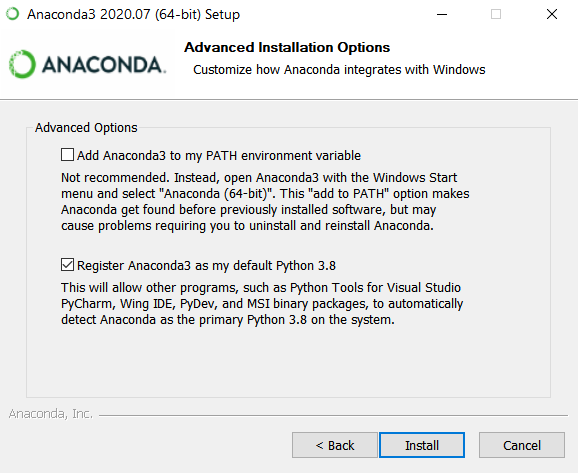
\includegraphics[width=0.7\linewidth]{Fig/conda.png}
			\caption{Anaconda installation}
			\label{fig:conda}
		\end{figure}
		\item Search \textbf{Anaconda Navigator} in the start menu and open jupyter notebook.
		\begin{figure}[h!]
			\centering
			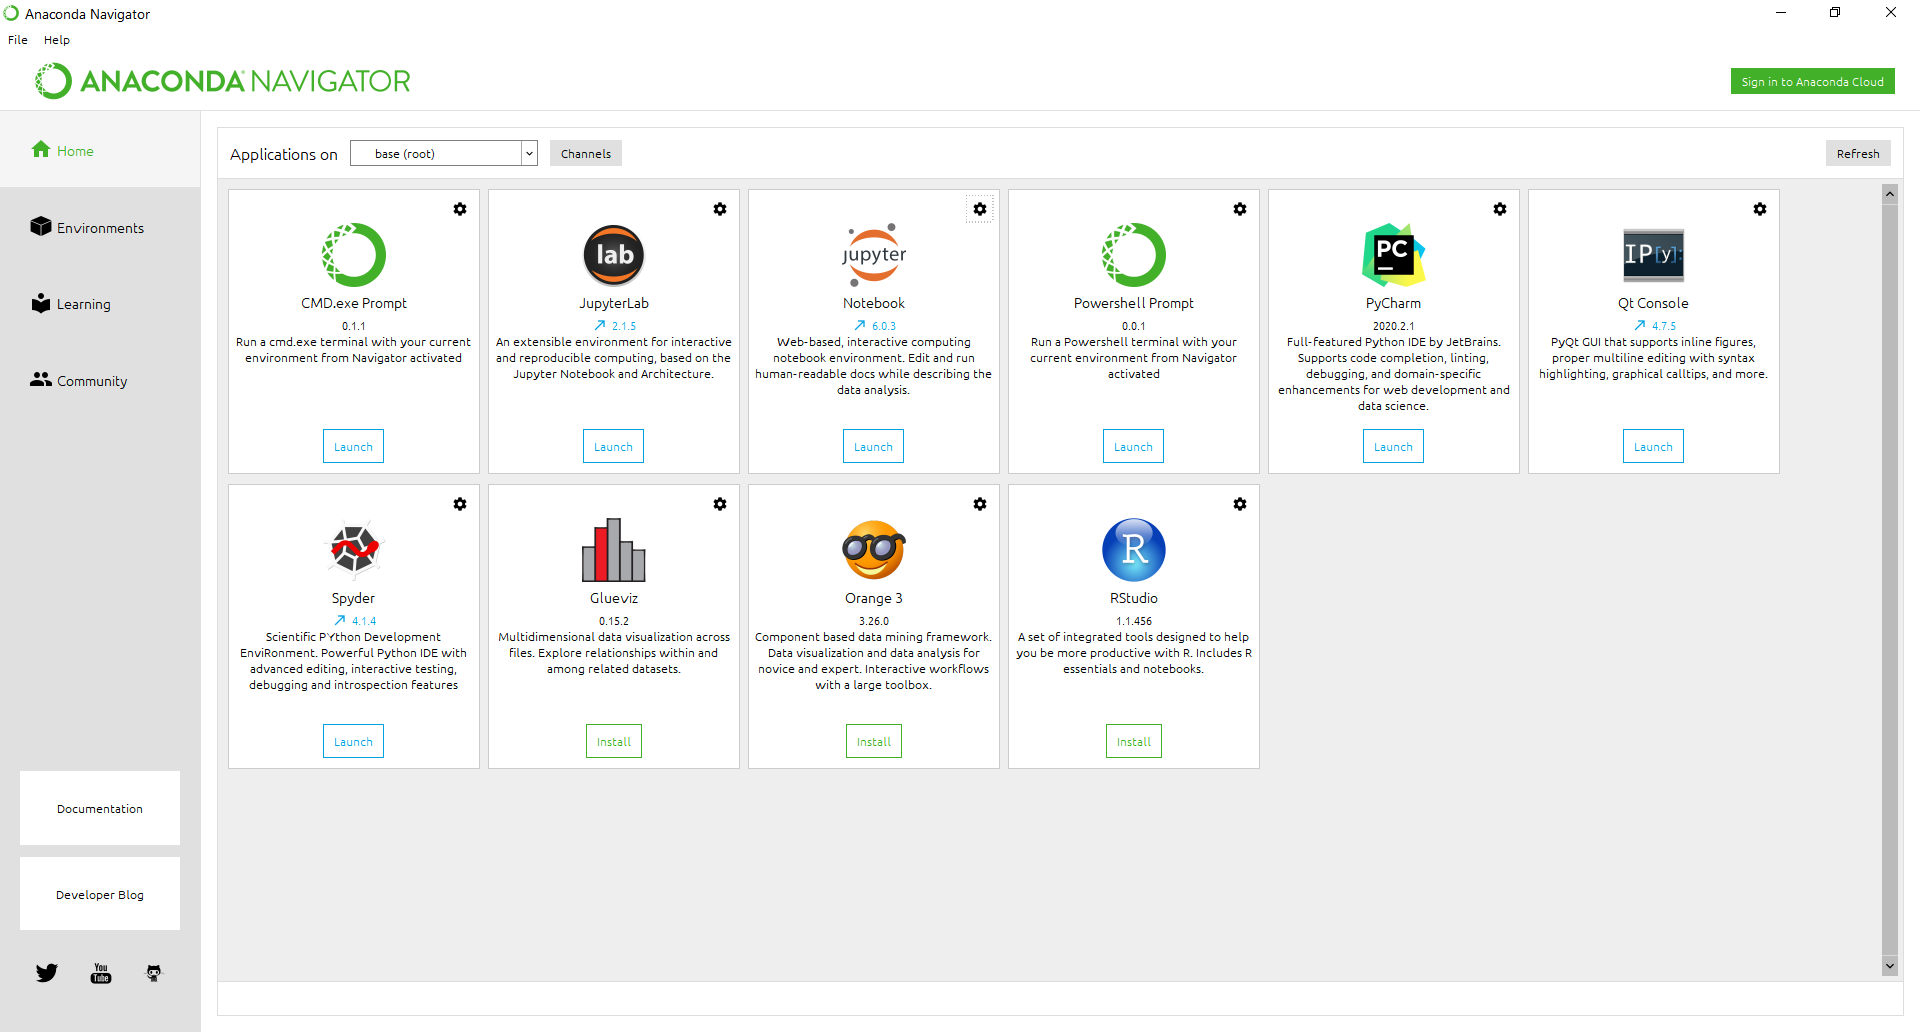
\includegraphics[width=\linewidth]{Fig/condaPrompt.png}
			\caption{Anaconda Navigator}
			\label{fig:condap}
		\end{figure}
		\begin{figure}[h!]
			\centering
			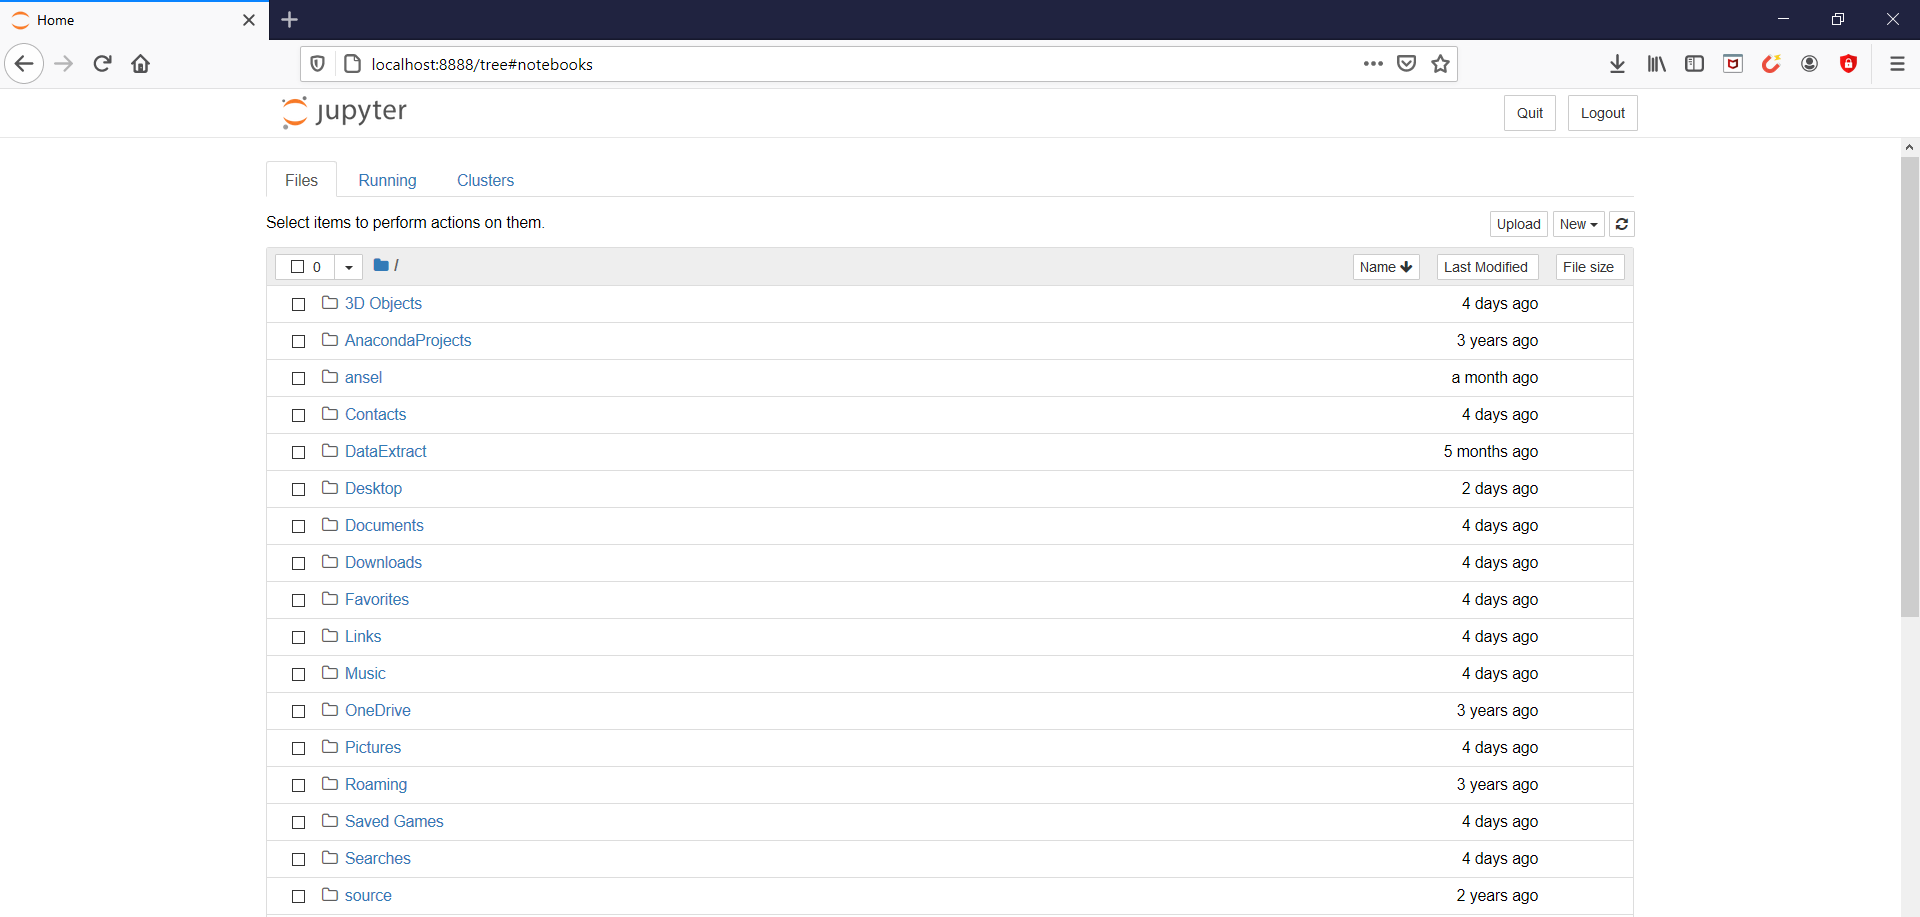
\includegraphics[width=\linewidth]{Fig/jupyter.png}
			\caption{Jupyter window}
			\label{fig:condap}
		\end{figure}
	
	\end{enumerate}

	\FloatBarrier

	\section*{2. Installing Gurobi}
	Gurobi is a commercial optimization solver. We will use it to solve various linear programs (LP). Here are the instructions to install gurobi and its license.
	
	\begin{enumerate}
		\item First go to the website \href{https://pages.gurobi.com/registration}{https://pages.gurobi.com/registration}.
		\item Make an account on this webpage. Select \textbf{Academic User} and fill out other details. Click on the confirmation email if needed.
		\begin{figure}[h!]
			\centering
			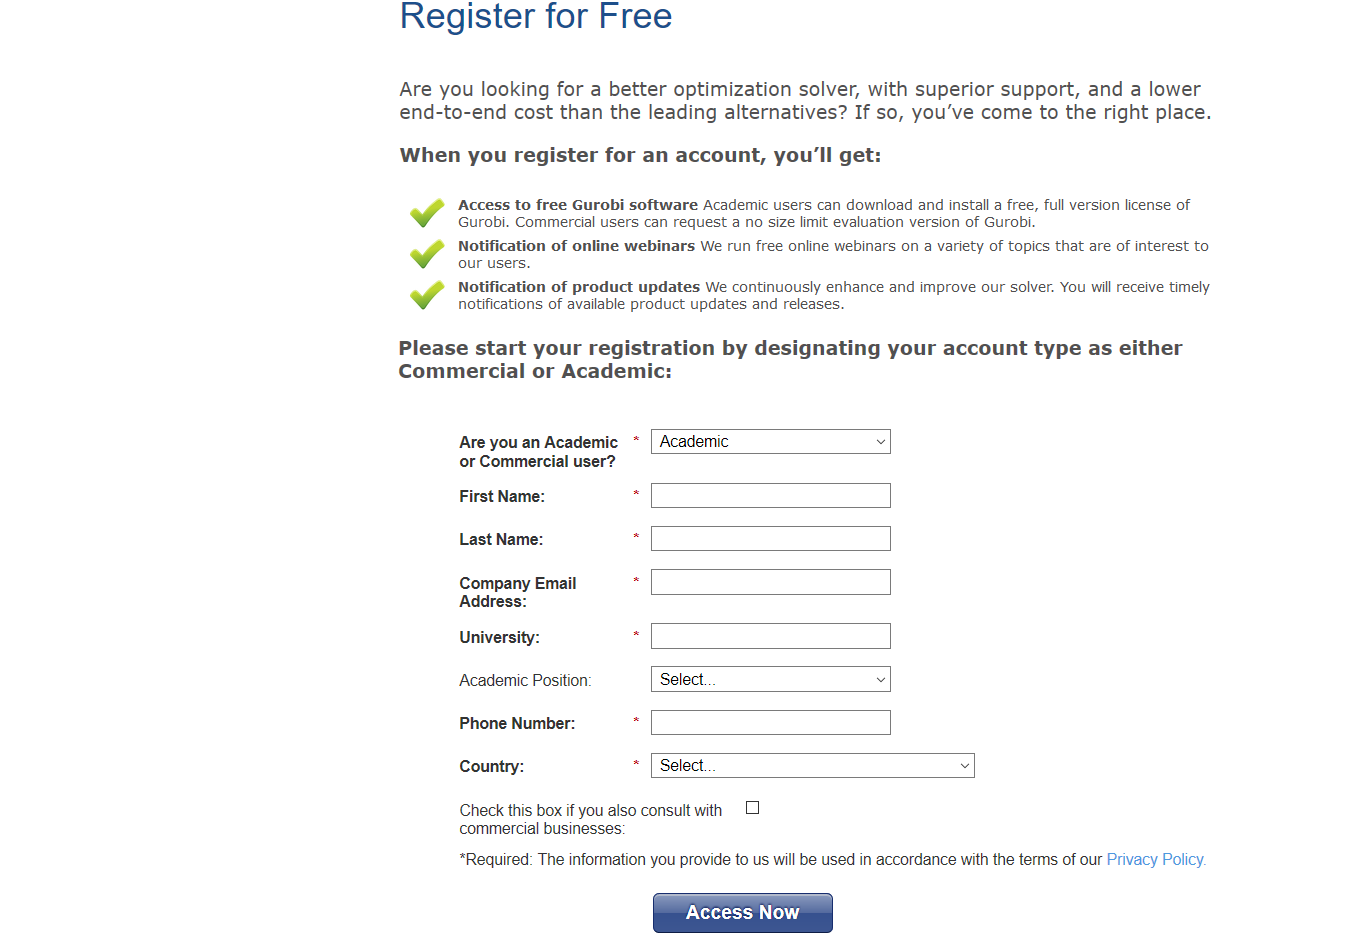
\includegraphics[width=\linewidth]{Fig/account.png}
			\caption{Gurobi registration}
			\label{fig:condap}
		\end{figure}
		\item Click on the link \href{https://www.gurobi.com/login/}{https://www.gurobi.com/login/} and login into your account.
		\item Now go to the website \href{https://www.gurobi.com/downloads/}{https://www.gurobi.com/downloads/}. Click on \textbf{Gurobi Optimizer} and the click on \textbf{I accept the end user license agreement}. Download the installer for appropriate OS and processor.
		\item Go to the download location and double click the msi installer. Click \textbf{Next}, check the user agreement and click \textbf{Next, Install} and \textbf{Finish}.
		
		\item Now go to \href{https://www.gurobi.com/downloads/end-user-license-agreement-academic/}{https://www.gurobi.com/downloads/end-user-license-agreement-academic/}. Click on \textbf{I accept these conditions}. Scroll down and copy the license key (See Figure \ref{fig:lic} below)
		
			\begin{figure}[h!]
			\centering
			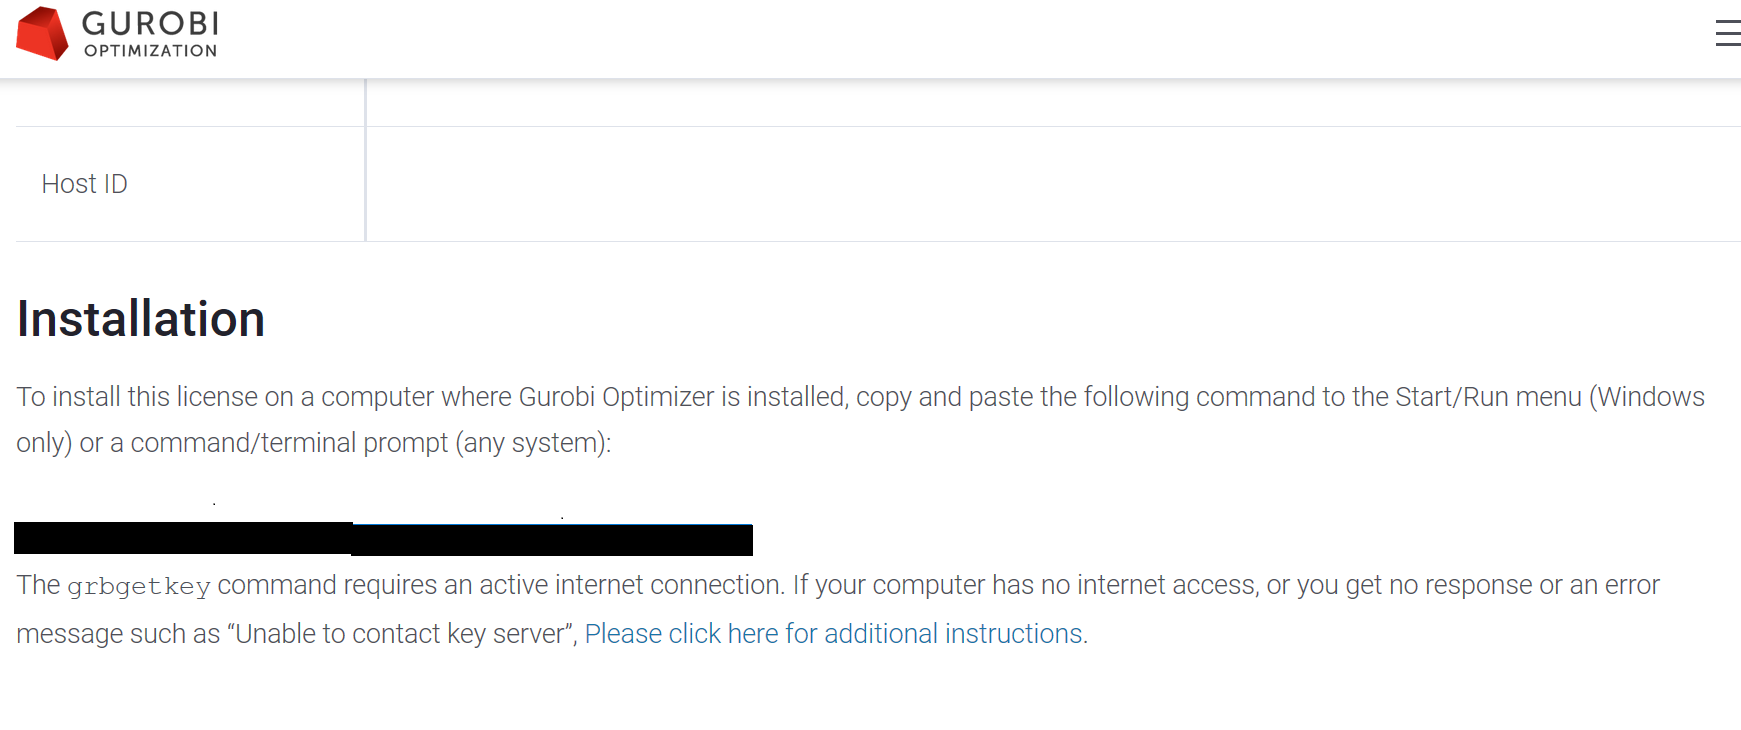
\includegraphics[width=\linewidth]{Fig/license.png}
			\caption{Gurobi license}
			\label{fig:lic}
		\end{figure}
	
		\item Now go to command prompt (Go to start menu and type cmd and hit enter). Paste the key and hit enter. You may need to type "y" and press enter.
		\item To install the python package \textbf{gurobipy}, open command line and change your directory to the Gurobi installation directory by using command \texttt{cd C:$\backslash$gurobi800$\backslash$ win64}. Now type \texttt{python setup.py install}
	
		
	\end{enumerate}
	

	
	
	
	
\end{document}
